\documentclass[English,t,% 't' (resp. 'c') places text vertically at top/center of the slides
% PDF settings
hyperref={%
    pdftitle={GM's Introduction},%
    pdfauthor={Guillaume Muller},%
    pdfsubject={GM's Introduction},%
    pdfkeywords={Presentation, Introduction}%
    },%
% To load many pre-defined color names
xcolor={pdftex,svgnames} % dvipsnames, dvipsnames*, svgnames, svgnames*, x11names,
]{beamer}

\usetheme{Copenhagen} % AnnArbor,Antibes,Bergen,Berkeley,Berlin,Boadilla,CambridgeUS,Copenhagen,Darmstadt,Dresden,Frankfurt,Goettingen,Hannover,Ilmenau,JuanLesPins,Luebeck,Madrid,Malmoe,Marburg,Montpellier,PaloAlto,Pittsburgh,Rochester,Singapore,Szeged,Warsaw,boxes,default

% Disable NavigationBar
\beamertemplatenavigationsymbolsempty

% Correct French/English indentation and splitting of words
\usepackage{babel}

% Correct management of accentuated chars in input file
\usepackage[utf8]{inputenc}

% Correct font for the generation of docs with accentuated chars
\usepackage[T1]{fontenc}      % Can handle hyphenation of words with accented characters
%%\usepackage[OT1]{fontenc}   % Might generated bad looking PDFs

% Access to many maths symbols
\usepackage{amsthm}
\usepackage{amsmath}
\usepackage{amsfonts}

% Insertion of images generated by external tools
\usepackage{graphicx}

% To generate pretty & scalable images directly in LaTeX
\usepackage{tikz}
% \draw[decorate,decoration={coil,amplitude=1.5cm, segment length=.4cm}] (5,5.5) -- (5,1.5) ;
\usetikzlibrary{decorations.text}
\usetikzlibrary{decorations.shapes}
\usetikzlibrary{decorations.pathmorphing,snakes}

\def\me{Guillaume \textsc{Muller}}

% To print numbers correctly
\usepackage{numprint}

% To position text blocks absolutely
\usepackage[absolute,overlay]{textpos}


%%%%%%%%%%%%%%%%%%%%%%%%%%%%%%%%%%%%%%%%%%%%%%%%%%%%%%%%%%%%%%%%%%%%%%
\begin{document}



%%%%%%%%%%%%%%%%%%%%%%%%%%%%%%%%%%%%%%%%%%%%%%%%%%%%%%%%%%%%%%%%%%%%%%%
\begin{frame}{Getting to know each other!}

\vspace{-.5cm}
%
  \begin{block}{Who am I?}
    { \footnotesize
      \begin{itemize}
        \item \textbf{Background}: PhD in Computer Science (Distributed AI)
        \item \textbf{Teaching} (@Telecom): MdC "LRU" [Prog., HPP, Secu, DevOps, Data]
        \item \textbf{Research} (@LabHC): Member of the Data Intelligence team
      \end{itemize}
    }
  \end{block}

  \begin{block}{What is my previous experience on the subject?}
    { \footnotesize
      \begin{itemize}
        \item PhD on P2P \& \textbf{Multi-Agent Systems} \hspace{1cm} 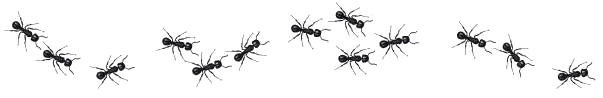
\includegraphics[height=3ex]{images02/ants2.png}\\[-2ex]
      \end{itemize}
      \begin{minipage}[c]{.45\linewidth}
        \begin{itemize}
          \item \textbf{Virtual Assistant} (2007!) \hfill 
\includegraphics[height=3ex]{images02/ggle_mic.png}    %: Speech \& Intention Recognition\ldots{} % Siri=2011 / Amazon Echo=2014 / GoogleHome/Assistant=2016
          \item \textbf{Serious Games}             \hfill 
\includegraphics[height=3ex]{images02/gamepad2.png}    %: Virtual Players
          \item \textbf{Solar Houses}              \hfill 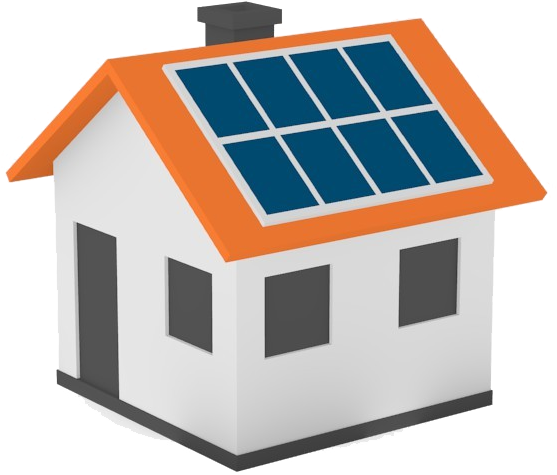
\includegraphics[height=3ex]{images02/solar_house.png} % Energy: Optimization of ...
        \end{itemize}
      \end{minipage}
      \begin{minipage}[c]{.45\linewidth}
        \begin{itemize}
          \item \textbf{Search Engines} \hfill 
\includegraphics[height=3ex]{images02/gsearch.jpeg}    %: Knowledge Extraction, Ranking, Preferences\ldots{}
          \item \textbf{Aircrafts}      \hfill 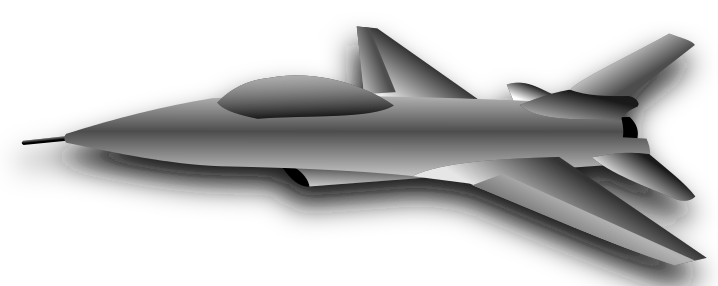
\includegraphics[height=3ex]{images02/aircraft.png}    %: predictive maintenance, failure predictions, crash prevention
          \item \textbf{Industry 4.0}   \hfill 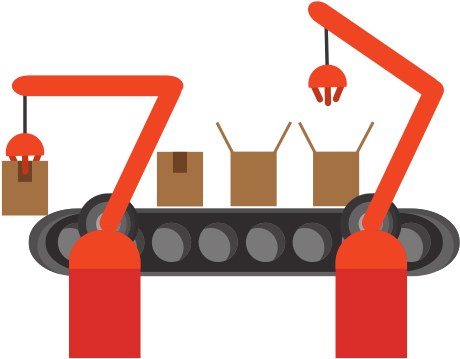
\includegraphics[height=3ex]{images02/industry_40.png} %: planification
        \end{itemize}
      \end{minipage}
    }
  \end{block}

  \begin{block}{Ongoing projects}
    { \footnotesize
      \begin{itemize}
        \item \textbf{Health Care}: BCI/EEGs, Suicide Prevention, Blood Transfusion
        \item[]~\\[-1cm] \hfill 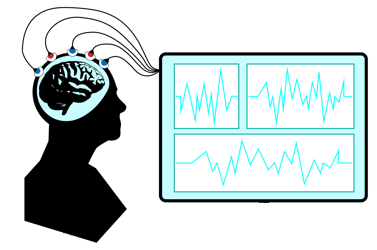
\includegraphics[height=4ex]{images02/bci1.png}
        \item \textbf{Privacy}: Federated Learning
      \end{itemize}
      }
  \end{block}

\end{frame}




%%%%%%%%%%%%%%%%%%%%%%%%%%%%%%%%%%%%%%%%%%%%%%%%%%%%%%%%%%%%%%%%%%%%%%
\begin{frame}{Who are you?}

\end{frame}


%%%%%%%%%%%%%%%%%%%%%%%%%%%%%%%%%%%%%%%%%%%%%%%%%%%%%%%%%%%%%%%%%%%%%%
\begin{frame}{Who am I?}

  \begin{itemize}
%
    \item Associate Professor in computer science, LRU
%
    \vspace{2em}
    \item \textbf{Teachings @TSÉ}
    \vspace{.5em}
    \begin{itemize}
      \item C/C++, Java, Spring
      \item Soft. Eng., Algo
      \item HPP, Secu, DevOps, Data
    \end{itemize}
%
    \vspace{2em}
    \item \textbf{Research @LHC}
    \vspace{.5em}
    \begin{itemize}
      \item Research in «~Data Intelligence team~»
      \item BCI/EEGs, Privacy
      \item (IA, Multi-Agent, BlockChain, QuantumML)
    \end{itemize}
%
  \end{itemize}

\begin{textblock*}{2cm}(8.7cm,6cm)%
  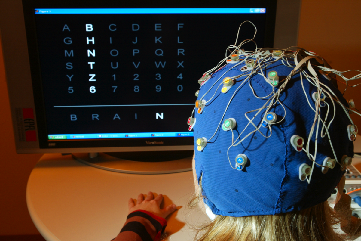
\includegraphics[width=1.7cm]{images02/bci3.png}
\end{textblock*}%

\begin{textblock*}{2cm}(11.5cm,6.5cm)%
  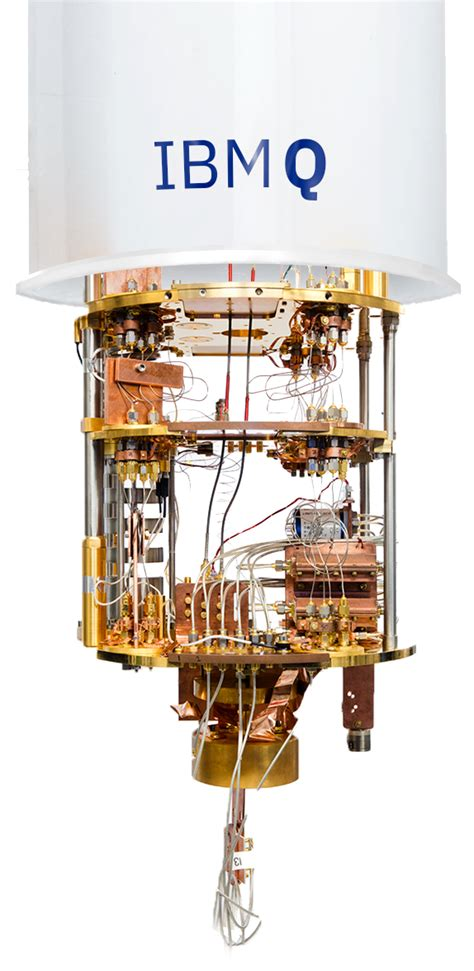
\includegraphics[width=.8cm]{images02/ibmq.jpeg}
\end{textblock*}%

\begin{textblock*}{2cm}(9.2cm,7.7cm)%
  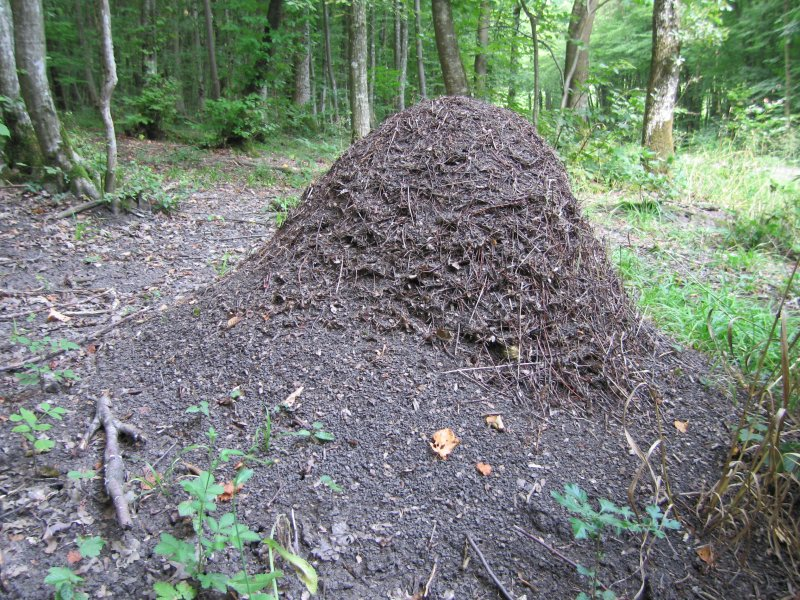
\includegraphics[width=2cm]{images02/ants.jpeg}
\end{textblock*}%

\end{frame}


\end{document}
